\documentclass[10pt,conference]{IEEEtran}
\usepackage{cite}
\usepackage{amsmath,amssymb}
\usepackage{booktabs}
\usepackage{array}
\usepackage{hyperref}
\usepackage{microtype}
\usepackage{xcolor}
\usepackage{graphicx}
\usepackage{listings}
\usepackage{float}
\usepackage{tcolorbox}
\tcbuselibrary{listings, skins, breakable}

% ---- YAML listing style ----
\lstdefinestyle{yaml}{
  basicstyle=\ttfamily\footnotesize,
  breaklines=true,
  breakatwhitespace=true,
  columns=flexible,
  keepspaces=true,
  commentstyle=\color{gray}\itshape,
  comment=[l]{\#},
  tabsize=2,
  showstringspaces=false,
}

\tcbset{
  codebox/.style={
    enhanced,
    breakable,
    colback=gray!4,
    colframe=gray!40,
    boxrule=0.5pt,
    arc=3pt,
    left=6pt, right=6pt, top=6pt, bottom=6pt,
    fonttitle=\small\bfseries,
    coltitle=black,
    attach title to upper={\par\smallskip},
    titlerule=0pt,
    toptitle=4pt,
    bottomtitle=4pt,
  }
}

\begin{document}

\title{Workflow as a Tool (WaaT): Structured Orchestration\\
for Production-Ready AI Agents}

\author{Bruno Ibanez Lopez\\
\textit{bruno.ibanezlopez@gmail.com}}

\maketitle

% ---------------------------------------------------------------
\begin{abstract}
Large language model (LLM) agents exhibit strong generalisation
across open-ended tasks, yet business process automation demands
the opposite: bounded, predictable, and traceable execution.  This
paper identifies the core limitations of existing orchestration
paradigms---code-driven state machines, prompt-driven flows, and
contemporary multi-agent frameworks---and proposes Workflow as a
Tool (WaaT) as a principled alternative.  In WaaT, business
processes are encoded as YAML definitions and exposed to a
super-agent through two dedicated runtime tool calls.  The model
may have global workflow context, but state advancement is
mediated by explicit current-state grounding, transition
validation, and mandatory reasoning.  Each state transition is
committed alongside the agent's justification, forming a complete
audit record.  The pattern yields systems that are structurally
verifiable before deployment, governable during execution, and
maintainable by non-engineers.  We situate WaaT within the mature tradition of
Business Process Management, describe the architecture and
validation framework, and present a prototype evaluation implemented
using the Strands agent framework on a 30-case adversarial synthetic
benchmark.  The evaluation is organised around two production-facing
claims: single-turn procedural correctness and resumable multi-turn
execution across user interaction boundaries.
\end{abstract}

\begin{IEEEkeywords}
LLM agents, agentic orchestration, business process automation,
workflow engineering, auditability, state machines, BPM.
\end{IEEEkeywords}
% ---------------------------------------------------------------


% ===============================================================
\section{Introduction}
% ===============================================================

The deployment of AI agents in operational business contexts
surfaces a fundamental tension.  Language models are trained to be
flexible, tolerant of ambiguity, and generative---properties
desirable in open-ended tasks such as research synthesis, but that
become liabilities when applied to structured business processes.
A service cancellation procedure, a billing dispute flow, or a
compliance verification sequence each requires not merely correct
execution but \emph{demonstrably} correct execution: the ability
to show, step by step, what decision was made and why.

When AI agents replace or augment human-operated processes, the
expectation of traceability does not diminish; if anything, it
increases.  An agent that fails silently, skips a compliance step,
or takes an undocumented branch is not merely a software
defect---it is a governance failure.

Existing orchestration approaches resolve this tension
inadequately.  Code-driven frameworks offer determinism at the
cost of maintainability; prompt-driven approaches offer flexibility
at the cost of reliability; multi-agent frameworks distribute
coordination logic in ways that resist inspection.  None provides
the combination of structural verifiability, mandatory reasoned
transitions, and business-owner legibility that production
deployments require.

We propose \emph{Workflow as a Tool} (WaaT), whose central
contribution is the combination of three ideas: (i) process logic
encoded as structured YAML; (ii) runtime-mediated workflow state
grounding and transition validation via tool calls; and (iii)
mandatory agent reasoning at every state transition, which
constitutes the audit trail.


% ===============================================================
\section{Background}
\label{sec:background}
% ===============================================================

The problem of executing structured business processes reliably
predates large language models by several decades.  WaaT is best
understood as extending a mature tradition rather than introducing
an entirely novel concept.

\subsection{Business Process Management and BPMN}

Business Process Management (BPM) is the discipline concerned with
the design, execution, and optimisation of organisational
processes~\cite{dumas2018fundamentals}.  Its canonical artefact,
the Business Process Model and Notation
(BPMN)~\cite{omg2013bpmn}, is an ISO-standardised language
(ISO/IEC~19510:2013) representing processes as directed graphs of
tasks, events, and gateways.  Production BPM engines---Camunda,
Zeebe, Flowable---execute BPMN definitions deterministically,
maintain full audit logs, and have been deployed in regulated
industries for over two decades.

WaaT can be understood as a YAML-native, LLM-aware re-expression
of the BPM execution model.  What BPM engines lack is any
mechanism for evaluating natural-language transition conditions or
capturing the \emph{reasoning} behind a branch decision.  The
agent fills precisely this gap.  WaaT does not replace BPM; it
extends it into the domain where transition conditions require
inference rather than rule evaluation.

\subsection{LLMs for Process Modelling}

Recent work has explored LLMs as modelling assistants for
generating and refining BPMN definitions.  Kourani et
al.~\cite{kourani2024promoai} demonstrate automated process model
creation and refinement from natural-language inputs.
Vidgof et al.~\cite{vidgof2023bpm} survey LLM applications in
BPM, identifying reliability challenges when outputs must satisfy
formal structural constraints.  This body of work focuses on LLMs
producing definitions for deterministic engines.  WaaT occupies a
complementary position: the LLM is the execution agent, consuming
a human-authored definition one step at a time.

\subsection{Code-Driven Orchestration}

Frameworks such as LangGraph~\cite{langgraph2024} represent
orchestration logic as explicit graphs in code, offering strong
reproducibility guarantees.  The principal limitation is
maintainability: every process change requires an engineer to
translate business intent into a graph modification, write
regression tests, and redeploy.  Code-driven systems also produce
audit artefacts of limited semantic value---execution logs record
\emph{what} path was taken but not \emph{why} a branch was
selected.

\subsection{Prompt-Driven Orchestration}

Embedding process logic in a system prompt lowers the barrier to
iteration but introduces reliability problems at scale.  Liu et
al.~\cite{liu2023lost} demonstrate empirically that model
performance on multi-step conditional reasoning degrades as a
function of context length---a finding with direct implications for
prompt-embedded process trees.  Natural-language condition
descriptions are also inherently ambiguous, with no formal
mechanism to detect discrepancies before deployment.

\subsection{ReAct and Planning-Based Agents}

ReAct~\cite{yao2023react} interleaves reasoning traces and actions
in a single sequence, producing partially interpretable execution
traces.  However, the action sequence emerges from in-context
reasoning at each step rather than a pre-specified graph,
precluding pre-deployment structural analysis.  Plan-and-Execute
variants~\cite{wang2024survey} separate planning from execution
but produce free-form natural-language plans rather than
machine-verifiable structures.

\subsection{Multi-Agent Frameworks}

AutoGen~\cite{wu2023autogen} and CrewAI~\cite{crewai2024} decompose
tasks across specialised agents communicating via message passing.
These excel at open-ended tasks requiring iterative refinement.
However, coordination logic is distributed across agent
configurations rather than centralised in a verifiable definition,
creating a traceability gap analogous to prompt-driven systems.

\subsection{Auditability in Agentic Systems}

The problem of constructing audit trails for LLM agent executions
has attracted recent attention.  Brady~\cite{brady2026springdrift}
presents Springdrift, a persistent runtime with append-only memory
and auditable axiom trails for normative safety gating.
Souza et al.~\cite{souza2025provenance} address workflow provenance
for scientific agents, proposing a reference architecture for
capturing causal relationships between actions and artefacts.
These works focus on infrastructure-level logging.  The key
distinction in WaaT is that the audit record is a mandatory
\emph{precondition} for state advancement, not a side-effect of
execution.

\subsection{Gap Analysis}

No existing paradigm simultaneously provides maintainability
without engineering overhead, full auditability of decision
rationale, structural verifiability prior to deployment, and
legibility for non-technical process owners.
Table~\ref{tab:gap} summarises coverage across these properties.

\begin{table}[ht]
\centering
\caption{Gap analysis across orchestration paradigms.}
\label{tab:gap}
\setlength{\tabcolsep}{4pt}
\renewcommand{\arraystretch}{1.15}
\begin{tabular}{lccccc}
\toprule
\textbf{Paradigm} &
\rotatebox{55}{\small\textbf{Maint.}} &
\rotatebox{55}{\small\textbf{Audit}} &
\rotatebox{55}{\small\textbf{Pre-deploy}} &
\rotatebox{55}{\small\textbf{Legibility}} &
\rotatebox{55}{\small\textbf{BPM roots}} \\
\midrule
BPMN engines  & Med  & Log   & Struct. & Med  & \checkmark \\
Code-driven   & Low  & Log   & Struct. & Low  & ---        \\
Prompt-driven & Med  & None  & None    & Med  & ---        \\
ReAct         & Med  & Part. & None    & Low  & ---        \\
AutoGen       & Med  & None  & None    & Low  & ---        \\
WaaT          & High & Full  & S.+Sem. & High & \checkmark \\
\bottomrule
\end{tabular}
\end{table}


% ===============================================================
\section{Workflow as a Tool}
\label{sec:architecture}
% ===============================================================

\subsection{Design Principles}

WaaT is founded on three design decisions.

\textbf{Separation of process definition and execution.}
Workflow logic is encoded as structured data, independent of both
the code that executes it and the prompt that drives it.  This
makes the definition independently readable, editable, and
analysable by automated tooling.

\textbf{Current-state grounding with global process context.}
The agent may receive the full workflow definition as global
instruction context, matching a realistic prompt-based baseline.
However, the actionable workflow state is still obtained through
\texttt{check\_workflow}: at each step the runtime identifies the
current state, exposes its valid outgoing transitions, and later
validates the requested update.  Global context helps the model
interpret process intent; the WaaT tools ensure that state
advancement remains grounded in the current executable state.

\textbf{Mandatory reasoned transitions.}
Every state advancement must be accompanied by an explicit
agent-generated justification.  This justification is persisted
and constitutes the audit record.  Calls that omit or trivially
populate the reasoning field are rejected at the tool level.

\subsection{System Components}

\textbf{Utility agents} are narrow, single-purpose, and stateless.
Each encapsulates one capability: invoking an external API,
retrieving a record, classifying a document.  They contain no
process logic and return structured, source-system-shaped results
to the super-agent: status, data, external references, errors, and
optionally a recommended next state.

\textbf{The super-agent} is the orchestrator.  It holds the
current workflow state, invokes utility agents as directed by the
active step, interprets their outputs against available
transitions, selects the next state, and calls
\texttt{update\_workflow} with its reasoning.  Its context is
grounded in the current step even when the full workflow is also
available as instruction context.

\textbf{Workflow sessions} persist the current state, accumulated
context, pending user requests, and the transition trace.  A WaaT
execution need not run to a terminal state in a single interaction:
it may suspend at an interaction boundary, such as a required user
confirmation, and later resume from the same workflow state.

\textbf{Workflow definitions} are YAML files.  Each defines a set
of states, an initial state, terminal states, and for each
non-terminal state: an action, its parameters, and transitions
with natural-language conditions.

\subsection{The Two Core Tools}

The super-agent is given access to exactly two workflow-related
tools.

\texttt{check\_workflow(state\_id)} returns the runtime
specification of the current state: the action to execute, its
parameters, and available transitions.  The model may have read
the full workflow definition, but this tool defines the current
executable state against which the next update will be validated.

{\sloppy\texttt{update\_workflow(current\_state\_id,~next\_state\_id,~reasoning)} advances the
workflow and persists the agent's reasoning.}  The
\texttt{reasoning} field is mandatory.  Calls that omit it are
rejected.  Reasoning is thus a precondition for advancement, not
a log entry appended after the fact.

Interaction states use the same state model but do not immediately
advance the workflow.  For example, a state whose action is
\texttt{request\_user\_confirmation} returns a user-facing prompt,
persists the pending request, and suspends execution.  When the
user responds, the super-agent resumes at that state and calls
\texttt{update\_workflow} with a reasoned transition grounded in
the user's response.


% ===============================================================
\section{Worked Example}
\label{sec:example}
% ===============================================================

\subsection{Workflow Definition}

Listing~\ref{lst:yaml} shows a representative YAML specification
for a service request routing workflow.  It illustrates
natural-language conditions legible to a business analyst,
multiple paths to an escalation terminal, and action parameters
that map to downstream service calls.

\begin{figure*}[b]
\begin{tcolorbox}[codebox, title={Listing 1: Service request routing workflow (partial).}]
\begin{lstlisting}[style=yaml]
workflow: SERVICE_REQUEST
initial_state: CLASSIFY_REQUEST
terminal_states:
  - REQUEST_COMPLETE
  - REQUEST_ESCALATED

states:
  CLASSIFY_REQUEST:
    action: call_classifier_agent
    action_params:
      customer_id:
      request_text:
    transitions:
      - to: HANDLE_ACCOUNT_QUERY
        condition: request relates to account information or balance
      - to: HANDLE_SERVICE_CHANGE
        condition: request is a service modification or upgrade
      - to: HANDLE_COMPLAINT
        condition: request contains a complaint or dissatisfaction
      - to: REQUEST_ESCALATED
        condition: request cannot be classified or contains sensitive content

  HANDLE_ACCOUNT_QUERY:
    action: call_account_agent
    action_params:
      customer_id:
      query_type:
    transitions:
      - to: REQUEST_COMPLETE
        condition: query answered and customer confirmed satisfied
      - to: HANDLE_COMPLAINT
        condition: customer dissatisfied with account information provided
      - to: REQUEST_ESCALATED
        condition: account data unavailable or agent cannot resolve
\end{lstlisting}
\end{tcolorbox}
\label{lst:yaml}
\end{figure*}

\subsection{Execution Trace}

An execution produces an ordered sequence of
\texttt{(state, result, next\_state, reasoning)} tuples.
Listing~\ref{lst:trace} shows a partial trace for a request
that routes through complaint handling.

\begin{figure*}[b]
\begin{tcolorbox}[codebox, title={Listing 2: Partial execution trace with mandatory reasoned transitions.}]
\begin{lstlisting}[style=yaml]
execution_id: exec-20250424-00312
workflow: SERVICE_REQUEST
trace:
  - state: CLASSIFY_REQUEST
    action_result:
      classification: COMPLAINT
      confidence: 0.91
    next_state_id: HANDLE_COMPLAINT
    reasoning: >
      Classifier returned COMPLAINT with confidence 0.91.
      Customer message contains explicit dissatisfaction.
      Selecting HANDLE_COMPLAINT per condition: request
      contains a complaint or expression of dissatisfaction.

  - state: HANDLE_COMPLAINT
    action_result:
      resolution_offered: true
      customer_accepted: true
    next_state_id: REQUEST_COMPLETE
    reasoning: >
      Resolution was offered and customer accepted.
      No further action required. Selecting REQUEST_COMPLETE.
\end{lstlisting}
\end{tcolorbox}
\label{lst:trace}
\end{figure*}

This trace is human-readable, reproducible, and tied to the
workflow definition in effect at execution time.  An auditor can
verify that each reasoning entry is consistent with the
corresponding transition condition.


% ===============================================================
\section{Pre-Deployment Validation}
\label{sec:validation}
% ===============================================================

Because workflow definitions are structured data, they admit
verification prior to any execution---a class of analysis
unavailable to code-based or prompt-based orchestration.

\subsection{Structural Analysis}

A structural pass operates on the directed graph implied by the
workflow's state and transition definitions.  It detects:
dead-end states not declared terminal; states unreachable from
the initial state; transitions referencing undefined states; and
execution paths with no route to any terminal state.  These checks
are computationally inexpensive, expressible as graph traversal
problems, and embeddable in a CI pipeline triggered by any change
to a workflow file.

\subsection{Semantic Analysis}

Structural correctness is necessary but insufficient.  A workflow
can be structurally sound yet contain transition conditions
ambiguous in ways that only manifest at runtime.  To address this,
a semantic pass submits each state's transition conditions to an
LLM evaluator assessing three properties per state:

{\sloppy
\begin{itemize}
  \item \textbf{Overlap}: whether any pair of conditions could be
  simultaneously satisfied for the same action result.
  \item \textbf{Gap}: whether realistic action outcomes exist not
  covered by any condition.
  \item \textbf{Vagueness}: whether any condition is too imprecise
  for an agent to reliably distinguish it from adjacent conditions.
\end{itemize}
}

The evaluator returns a numeric ambiguity score
(0\,=\,unambiguous, 100\,=\,highly problematic), a list of
identified issues, and a recommended reformulation for states
exceeding a threshold.  Table~\ref{tab:validation} shows
representative findings from both passes.

\begin{table}[ht]
\centering
\caption{Representative findings from structural and semantic
validation passes.}
\label{tab:validation}
\setlength{\tabcolsep}{3pt}
\renewcommand{\arraystretch}{1.15}
\begin{tabular}{p{1.2cm}p{2.2cm}p{4.0cm}}
\toprule
\textbf{Pass} & \textbf{Type} & \textbf{Example finding} \\
\midrule
Structural & Dead-end state &
  Node with empty transitions not declared terminal \\
Structural & Broken reference &
  Transition targeting undefined state name \\
Semantic & Overlap [60] &
  Two conditions both satisfiable for same input \\
Semantic & Gap [70] &
  No condition handles dissatisfied customer outcome \\
Semantic & Vagueness [45] &
  ``issue resolved'' without specifying resolution criteria \\
\bottomrule
\end{tabular}
\end{table}

\subsection{Stakeholder Reporting}

Validation output is produced in two forms.  A technical report
provides the full structural graph, per-state ambiguity scores,
and issue descriptions.  A stakeholder report renders the workflow
as a readable diagram with plain-language annotations, enabling
non-technical process owners to review and sign off the
specification before deployment.  The goal is not merely that
workflows \emph{can} be read by business stakeholders, but that
they \emph{are} read and approved as part of a governance gate.


% ===============================================================
\section{Comparative Analysis}
\label{sec:comparison}
% ===============================================================

Table~\ref{tab:comparison} compares WaaT against the paradigms in
Section~\ref{sec:background} across eleven criteria.  We
explicitly include criteria on which WaaT does not lead to ensure
analytical completeness.

\begin{table*}[ht]
\centering
\caption{Orchestration paradigm comparison. \textbf{Bold}: leading paradigm(s). \textit{Italic}: WaaT trails.}
\label{tab:comparison}
\setlength{\tabcolsep}{4pt}
\renewcommand{\arraystretch}{1.15}
\begin{tabular}{lccccccc}
\toprule
\textbf{Criterion} &
\rotatebox{55}{\small BPMN} &
\rotatebox{55}{\small Code} &
\rotatebox{55}{\small Prompt} &
\rotatebox{55}{\small ReAct} &
\rotatebox{55}{\small AutoGen} &
\rotatebox{55}{\small Asst.} &
\rotatebox{55}{\small\textbf{WaaT}} \\
\midrule
Maintainability      & M & L & M & M & M & M & \textbf{H} \\
Auditability         & Log & Log & --- & Part & --- & --- & \textbf{Full} \\
Reasoned transitions & -- & -- & -- & Part & -- & -- & \textbf{Yes} \\
Biz.\ legibility     & M & L & M & L & L & M & \textbf{H} \\
Deep branching       & \textbf{H} & \textbf{H} & L & M & M & M & \textbf{H} \\
Context efficiency   & \textbf{n/a} & \textbf{n/a} & Poor & Poor & Poor & Poor & \textbf{Bnd} \\
Pre-deploy valid.    & Str & Str & -- & -- & -- & -- & \textbf{S+Sm} \\
Eng.\ dependency     & M & H & \textbf{L} & \textbf{L} & M & \textbf{L} & \textbf{L} \\
BPM alignment        & \textbf{Yes} & -- & -- & -- & -- & -- & \textbf{Yes} \\
\midrule
Open-ended fit       & -- & L & M & \textbf{H} & \textbf{H} & \textbf{H} & \textit{L} \\
Latency / step       & \textbf{L} & \textbf{L} & \textbf{L} & M & M & M & \textit{M} \\
Authoring cost       & H & H & \textbf{L} & \textbf{L} & \textbf{L} & \textbf{L} & M \\
\bottomrule
\multicolumn{8}{l}{\scriptsize H=High, M=Med, L=Low, Bnd=Bounded,
Str=Structural, S+Sm=Structural+Semantic}
\end{tabular}
\end{table*}

\subsection{Where WaaT Leads}

\paragraph{Auditability and reasoned transitions.}
The mandatory \texttt{reasoning} field produces an audit record
qualitatively different from any competing paradigm.  Code-driven
systems and BPMN engines record execution paths but not decision
rationale.  ReAct produces reasoning traces interleaved with
actions in a sequence not designed for business auditor inspection.
WaaT externalises each transition decision as a named, persisted,
human-readable artefact.  Crucially, reasoning is a
\emph{precondition} for advancement: the system cannot proceed
without it~\cite{brady2026springdrift}.

\paragraph{Pre-deployment validation.}
Structural graph analysis and LLM-based semantic evaluation of
condition quality are both possible before any execution.  BPMN
engines support structural analysis but not semantic evaluation of
condition ambiguity~\cite{vidgof2023bpm}.  Prompt-driven and
agent-based frameworks provide neither.

\paragraph{BPM standards alignment.}
WaaT definitions are semantically aligned with the BPM tradition
and legible to analysts trained in process modelling.  The broader
body of BPM research on process verification, conformance
checking, and process mining is directly applicable.

\subsection{Where WaaT Trails}

\paragraph{Open-ended task fit.}
WaaT is not appropriate when the execution path cannot be
determined in advance.  ReAct, AutoGen, and Assistants API
tool-use are better suited to exploratory tasks.  This is a
deliberate design constraint: WaaT optimises for predictability
and governance over generality.

\paragraph{Latency.}
Each WaaT step requires at minimum two tool calls in addition to
utility agent invocations.  In latency-sensitive automations this
cost should be evaluated against the auditability benefit.
Per-step latency is bounded by step complexity rather than
workflow length.

\paragraph{Initial authoring cost.}
Authoring YAML with well-specified transition conditions requires
upfront effort that prompt-driven approaches do not.
The pre-deployment validation tooling partially offsets this by
surfacing specification errors early.  LLM-based process modelling
tools~\cite{kourani2024promoai} represent a promising direction
for automating initial definition generation.


% ===============================================================
\section{Applicability and Limitations}
\label{sec:applicability}
% ===============================================================

WaaT is most effective when: process logic can be specified in
advance; branching depends on structured data returned by utility
agents; step-level audit records are required; and process
ownership should reside with business stakeholders.  Concrete
domains include regulated customer service flows, multi-step
approval chains, compliance verification sequences, and service
lifecycle management.

The pattern is not appropriate for open-ended tasks.  WaaT itself
is also unnecessary for single-action automations requiring no
orchestration, although a production request orchestrator may route
such requests directly to utility agents while reserving WaaT for
procedural execution.

Three limitations warrant explicit acknowledgement.

\paragraph{Audit quality is bounded by specification quality.}
Vague transition conditions yield formally present but
substantively uninformative reasoning.  The semantic validation
pass surfaces these cases before deployment but does not
eliminate the need for careful authorship.

\paragraph{Loop termination requires deliberate memory design.}
When a state may transition back to itself, the YAML specification
alone cannot enforce a maximum iteration count.  Contemporary agent
frameworks provide episodic and working memory strategies---such as
those available in Amazon Bedrock AgentCore---that can persist
visit counts and prior action results across \texttt{check\_workflow}
calls.  However, this memory must be explicitly wired into the
workflow infrastructure; it does not arise automatically from the
WaaT pattern itself.  Authors of looping states should either
inject a visit counter into the \texttt{check\_workflow} response
at the infrastructure level, or declare an explicit maximum-attempts
terminal transition in the YAML definition, ensuring the agent has
a principled exit condition regardless of the memory strategy in
use.

\paragraph{A new artefact class requires new governance practices.}
YAML workflow files are business-critical artefacts requiring
version control, access control, and structured review
processes---including the stakeholder sign-off described in
Section~\ref{sec:validation}.


% ===============================================================
\section{Evaluation}
\label{sec:evaluation}
% ===============================================================

\subsection{Production Motivation}

Production customer-service agents rarely operate over a single
linear procedure.  In practice, an enterprise support agent must
coordinate multiple workflows---assurance, billing, cancellations,
customer care, ticket updates, account administration, and service
information retrieval.  Each workflow may contain many states,
conditional transitions, tool dependencies, authorisation gates,
escalation paths, and recovery actions.  Encoding this procedural
complexity directly into a system prompt is brittle: the prompt
grows with every workflow, the model must reason over irrelevant
states, and transition validity is enforced only by
instruction-following rather than by an explicit runtime mechanism.
This becomes especially problematic when different workflows share
surface-level language but require different operational controls,
such as a cancellation request that also requires billing
authorisation, save-offer checks, service inventory lookup, and
case creation.

WaaT addresses this problem by making workflow state an executable
runtime object rather than only static prompt text.  In the
evaluation, both WaaT and the prompt baseline receive the complete
workflow definition as global context.  The decisive difference is
that WaaT also exposes two workflow-control tools.
\texttt{check\_workflow} grounds the model in the current state's
action, action parameters, and valid outgoing transitions.
\texttt{update\_workflow} advances the workflow only when the
requested transition is valid and the model supplies non-trivial
reasoning.  This design makes the workflow executable,
inspectable, and enforceable at runtime.

\subsection{Implementation}

The prototype is implemented using Strands, matching the agent
framework used in our production environment.  The WaaT control
functions \texttt{check\_workflow} and \texttt{update\_workflow}
are implemented as Strands \texttt{@tool} functions and attached
to a Strands super-agent.  The implementation comprises a YAML
workflow loader and state-graph validator (\texttt{workflow.py}),
the two core Strands tool definitions and workflow session state
(\texttt{tools.py}), the resumable super-agent loop
(\texttt{agent.py}), production-shaped result contracts
(\texttt{contracts.py}), deterministic mock utility agents
(\texttt{mock\_agents.py}), a stepwise prompt baseline
(\texttt{baseline.py}), and a reasoning-quality evaluator
(\texttt{evaluator.py}).

For reproducibility, the evaluation uses deterministic mock
utility agents while invoking the workflow-control tools directly.
The transition choices, prompt baseline, and reasoning-quality
scoring are Bedrock-backed model calls; the source-system responses
are deterministic so that differences reflect orchestration
behaviour rather than external API variance.  The
\texttt{update\_workflow} tool enforces a minimum reasoning length
at the tool level: calls with fewer than twenty words in the
reasoning field are rejected and the agent must retry with a
substantive justification.  A separate multi-turn workflow fixture
includes a \texttt{request\_user\_confirmation} state; a
Bedrock-backed runner executes the first turn until suspension,
resumes with the user's confirmation response, and records the
resulting path.

\subsection{Experimental Setup}
\label{subsec:waat-experimental-setup}

We evaluated WaaT on 30 synthetic customer-service requests
covering account queries, service changes, complaints, and
ambiguous or sensitive edge cases.  Cases span four categories:
eight account-query cases (mixed satisfied and dissatisfied
outcomes), eight service-change cases (mixed completed and
escalated), eight complaint cases (mixed resolved and escalated),
and six edge cases (ambiguous, sensitive, or unclassifiable
requests).

Each case specifies a synthetic \texttt{customer\_id}, a realistic
free-text \texttt{request\_text}, an
\texttt{expected\_terminal\_state} (\textsc{request\_complete} or
\textsc{request\_escalated}), and an \texttt{expected\_path}
listing the intended state sequence.

\paragraph{Evaluation methodology.}
The naive evaluation of WaaT on clean, well-formed requests
achieves 100\% terminal accuracy---consistent with the behaviour
observed in typical agent demonstrations.  We deliberately
rejected this methodology.  Reporting best-case performance on
unambiguous inputs characterises the ceiling of the architecture
but provides no information about how it behaves at production
boundary conditions, where requests are ambiguous, utility-agent
signals are imperfect, and classification confidence is
unreliable.  The benchmark presented here is therefore designed
as a stress test: cases are constructed to induce realistic
failure modes, and the reported figures reflect performance under
those conditions.  The 100\% clean-path result and the adversarial
benchmark figures together bound the expected production accuracy
range, with the true operating point depending on the cleanliness
of the real request distribution.

\paragraph{Non-oracle mock agents.}
The benchmark intentionally includes adversarial cases that
resemble production boundary conditions.  An earlier
implementation passed each case's \texttt{expected\_path}
directly to the mock utility agents, effectively handing the
system the answer key and producing artificially perfect accuracy.
The benchmark presented here removes this oracle dependency.  Each
mock agent makes an independent local decision from request
metadata and its own output fields: the classifier routes based on
category signals in the request text; the account, service, and
complaint agents decide from \texttt{query\_type},
\texttt{change\_type}, \texttt{complaint\_type}, and
\texttt{edge\_type} fields respectively.

Fixed reproducible hard cases ensure the benchmark is not
answer-key driven:
\begin{itemize}
  \item Account requests with strong dissatisfaction cues are
        routed directly to complaint handling rather than account
        resolution.
  \item Ambiguous edge cases are over-classified into account or
        service paths instead of being escalated at classification
        time.
  \item One service-change case is incorrectly treated as
        processable and marked complete rather than escalated for
        manual approval.
\end{itemize}

\paragraph{Baseline.}
We compare WaaT against a stepwise workflow-as-prompt baseline.
Both conditions receive the complete workflow definition as static
instruction context.  At each step, the baseline receives the
current case context and utility-agent output, then predicts the
next state without calling \texttt{check\_workflow} or
\texttt{update\_workflow}.  This represents a common alternative
design: the model is instructed to follow the complete procedure,
but transitions are not externally validated and reasoning is not
a precondition for state advancement.  WaaT receives the same
global workflow context but must advance through the runtime tools.
Token counts for both conditions are recorded using the Anthropic
API's usage fields and interpreted as execution cost or overhead,
not as the primary benefit.

\subsection{Metrics}

We report five metrics across the 30 test cases:

\begin{enumerate}
  \item \textbf{Transition accuracy}: proportion of individual
        \texttt{update\_workflow} calls in which the agent selected
        the correct \texttt{next\_state\_id}.
  \item \textbf{Path accuracy}: proportion of cases in which the
        full state sequence matched \texttt{expected\_path} exactly.
  \item \textbf{Terminal state accuracy}: proportion of cases in
        which the workflow reached \texttt{expected\_terminal\_state},
        regardless of intermediate path.
  \item \textbf{Reasoning quality}: each \texttt{update\_workflow}
        reasoning field is scored on a 1--5 scale by a second LLM
        call (1\,=\,trivial or empty, 3\,=\,adequate,
        5\,=\,specific and well-grounded in workflow evidence).
        We report mean score and distribution.
  \item \textbf{Token usage}: mean prompt-plus-completion
        tokens per case and per step for WaaT, mean tokens per
        case for the stepwise prompt baseline, and the aggregate
        WaaT-versus-baseline token delta.  This is reported as
        cost/overhead, not as the central success criterion.
\end{enumerate}

\subsection{Results}
\label{sec:results}

\begin{table}[t]
\centering
\caption{Single-turn WaaT results compared with a stepwise
workflow-as-prompt baseline across 30 synthetic service requests.
Values should be regenerated after any prompt or baseline change.}
\label{tab:waat-results}
\begin{tabular}{lc}
\hline
\textbf{Metric} & \textbf{Result} \\
\hline
WaaT transition accuracy             & pending rerun \\
Prompt baseline transition accuracy  & pending rerun \\
WaaT path accuracy                   & pending rerun \\
Prompt baseline path accuracy        & pending rerun \\
WaaT terminal state accuracy         & pending rerun \\
Prompt baseline terminal accuracy    & pending rerun \\
Mean reasoning quality               & pending rerun \\
Mean WaaT tokens / step              & pending rerun \\
Mean prompt baseline tokens / case   & pending rerun \\
WaaT vs baseline token delta         & pending rerun \\
\hline
\end{tabular}
\end{table}

Table~\ref{tab:waat-results} is populated by
\texttt{run\_evaluation.py}.  Because both conditions receive the
full workflow definition as instruction context, the reported
values must be regenerated whenever prompts, mock payloads, or
workflow definitions change.  The intended comparison is whether
WaaT's externally validated transitions, explicit current-state
grounding, and persisted reasoning improve procedural governance
when intermediate utility-agent signals are ambiguous or locally
incomplete.

The distinction between path accuracy and terminal accuracy is
important for workflow orchestration.  Terminal correctness
captures whether the request was ultimately completed or escalated
correctly, whereas path accuracy captures whether the agent
followed the intended procedural route.  The trace-level outputs
are used to inspect whether failures arise from classification
ambiguity, over-confident utility-agent outputs, or locally
plausible transitions that are globally suboptimal.

Reasoning quality is scored separately from path correctness.  This
supports the auditability claim: even when a transition is wrong,
the persisted justification can reveal whether the error came from
weak evidence, ambiguous state conditions, or a misleading
utility-agent result.

The single-turn evaluation records token usage for both conditions.
Since WaaT and the baseline both receive the full workflow
definition, token measurements should be interpreted as the cost or
overhead of adding runtime workflow-control tools, not as a claim
that WaaT primarily reduces prompt context.  If the prompt baseline
matches or exceeds WaaT accuracy on some generated workflows, this
is consistent with the experimental design: global context can help
reasoning, while WaaT's contribution is runtime validation,
auditability, and resumable state control.

\subsection{Production Implications}

The production motivation for WaaT is stronger than the synthetic
benchmark alone suggests.  Real deployments contain more
workflows, more states per workflow, more utility-agent
dependencies, and more cross-workflow handoffs than the small
service-request workflow used in this experiment.  In such
settings, workflow-as-prompt approaches require the prompt to
carry an increasingly large procedural burden.  As the number of
workflows grows, the model must identify the relevant workflow,
ignore irrelevant branches, remember transition constraints, and
apply policy or authorisation gates.  Even when the full workflow
is present in context, prompt-only control still lacks a runtime
mechanism that can reject invalid state updates or require
transition reasoning before advancement.

WaaT shifts the decisive control point from prompt text into
executable tooling.  Workflow state becomes an operational object
that the agent queries and updates, rather than only background
prose that the agent is expected to follow.  This makes procedural
behaviour more modular, auditable, and scalable: new workflows can
be added as YAML definitions; transition validation is enforced by
code; and each update is logged with explicit reasoning.
Critically, when failures do occur they are concentrated at known
classification boundaries, logged with the reasoning that produced
them, and therefore recoverable---a stronger operational guarantee
than a higher-accuracy system that fails silently or
unpredictably.  These properties are particularly important for
enterprise agent systems, where production-readiness requires
moving beyond prompt-only control toward architectures that
combine language-model flexibility with software-enforced process
boundaries.

The same state model supports conversational execution.  In the
multi-turn service-change fixture, WaaT pauses at a confirmation
state, returns a prompt to the user, persists the pending request,
and resumes after the user's reply.  This keeps the central
runtime guarantee intact across turns: the resumed transition is
still validated against the current state's outgoing edges and is
still accompanied by explicit reasoning.


% ===============================================================
\section{Conclusion}
\label{sec:conclusion}
% ===============================================================

We have presented Workflow as a Tool, an architectural pattern for
LLM-based process automation that addresses the principal
shortcomings of code-driven, prompt-driven, and multi-agent
orchestration paradigms.  By encoding business logic as YAML
workflow definitions, exposing executable workflow state through
two well-defined tool interfaces, and requiring every state
transition to carry an explicit agent-generated justification,
WaaT produces agent systems that are simultaneously flexible,
auditable, and maintainable by non-engineers.

WaaT is positioned within the mature tradition of Business Process
Management.  The core contribution relative to classical BPM
execution is the replacement of deterministic rule evaluation with
LLM-based inference at transition points, combined with the
elevation of transition reasoning from an optional log entry to a
mandatory precondition for state advancement.  This single
constraint distinguishes WaaT from a BPMN engine with an LLM
interpreter, and from a logging wrapper around an existing agent
framework.

A prototype evaluation implemented using the Strands agent
framework is organised around two claims: single-turn procedural
correctness on a compact adversarial service-request benchmark,
and resumability across a user-confirmation boundary.  The reported
metrics should be regenerated after changes to prompts, baseline
structure, or utility-agent payload contracts.

The implementation also demonstrates how the same primitive can
support resumable, multi-turn workflow execution through explicit
interaction states.  Broader request-level orchestration---for
example routing a user request to a direct utility-agent call,
a WaaT workflow, or a hybrid path---remains outside the evaluated
kernel and is left to future work.

The most consequential property of the pattern may be
organisational rather than technical: it returns ownership of
process logic to the business stakeholders who possess the
relevant domain knowledge.  As LLM agents move from experimental
deployments into production infrastructure, the ability to satisfy
governance requirements---not merely functional ones---will
determine which architectures prove durable.

Future work includes empirical evaluation of reasoning quality
across agent models, formal characterisation of completeness
properties achievable through YAML-based specification,
investigation of hybrid approaches combining structured YAML steps
with sub-step free-form reasoning, and integration with LLM-based
process modelling tools to reduce initial authoring cost.


% ===============================================================
\section*{Figure 1: Workflow State Diagram}
% ===============================================================

Figure~\ref{fig:workflow} renders the
\texttt{SERVICE\_REQUEST} workflow of Listing~\ref{lst:yaml}
as a directed labelled graph.

\begin{figure*}[t]
\centering
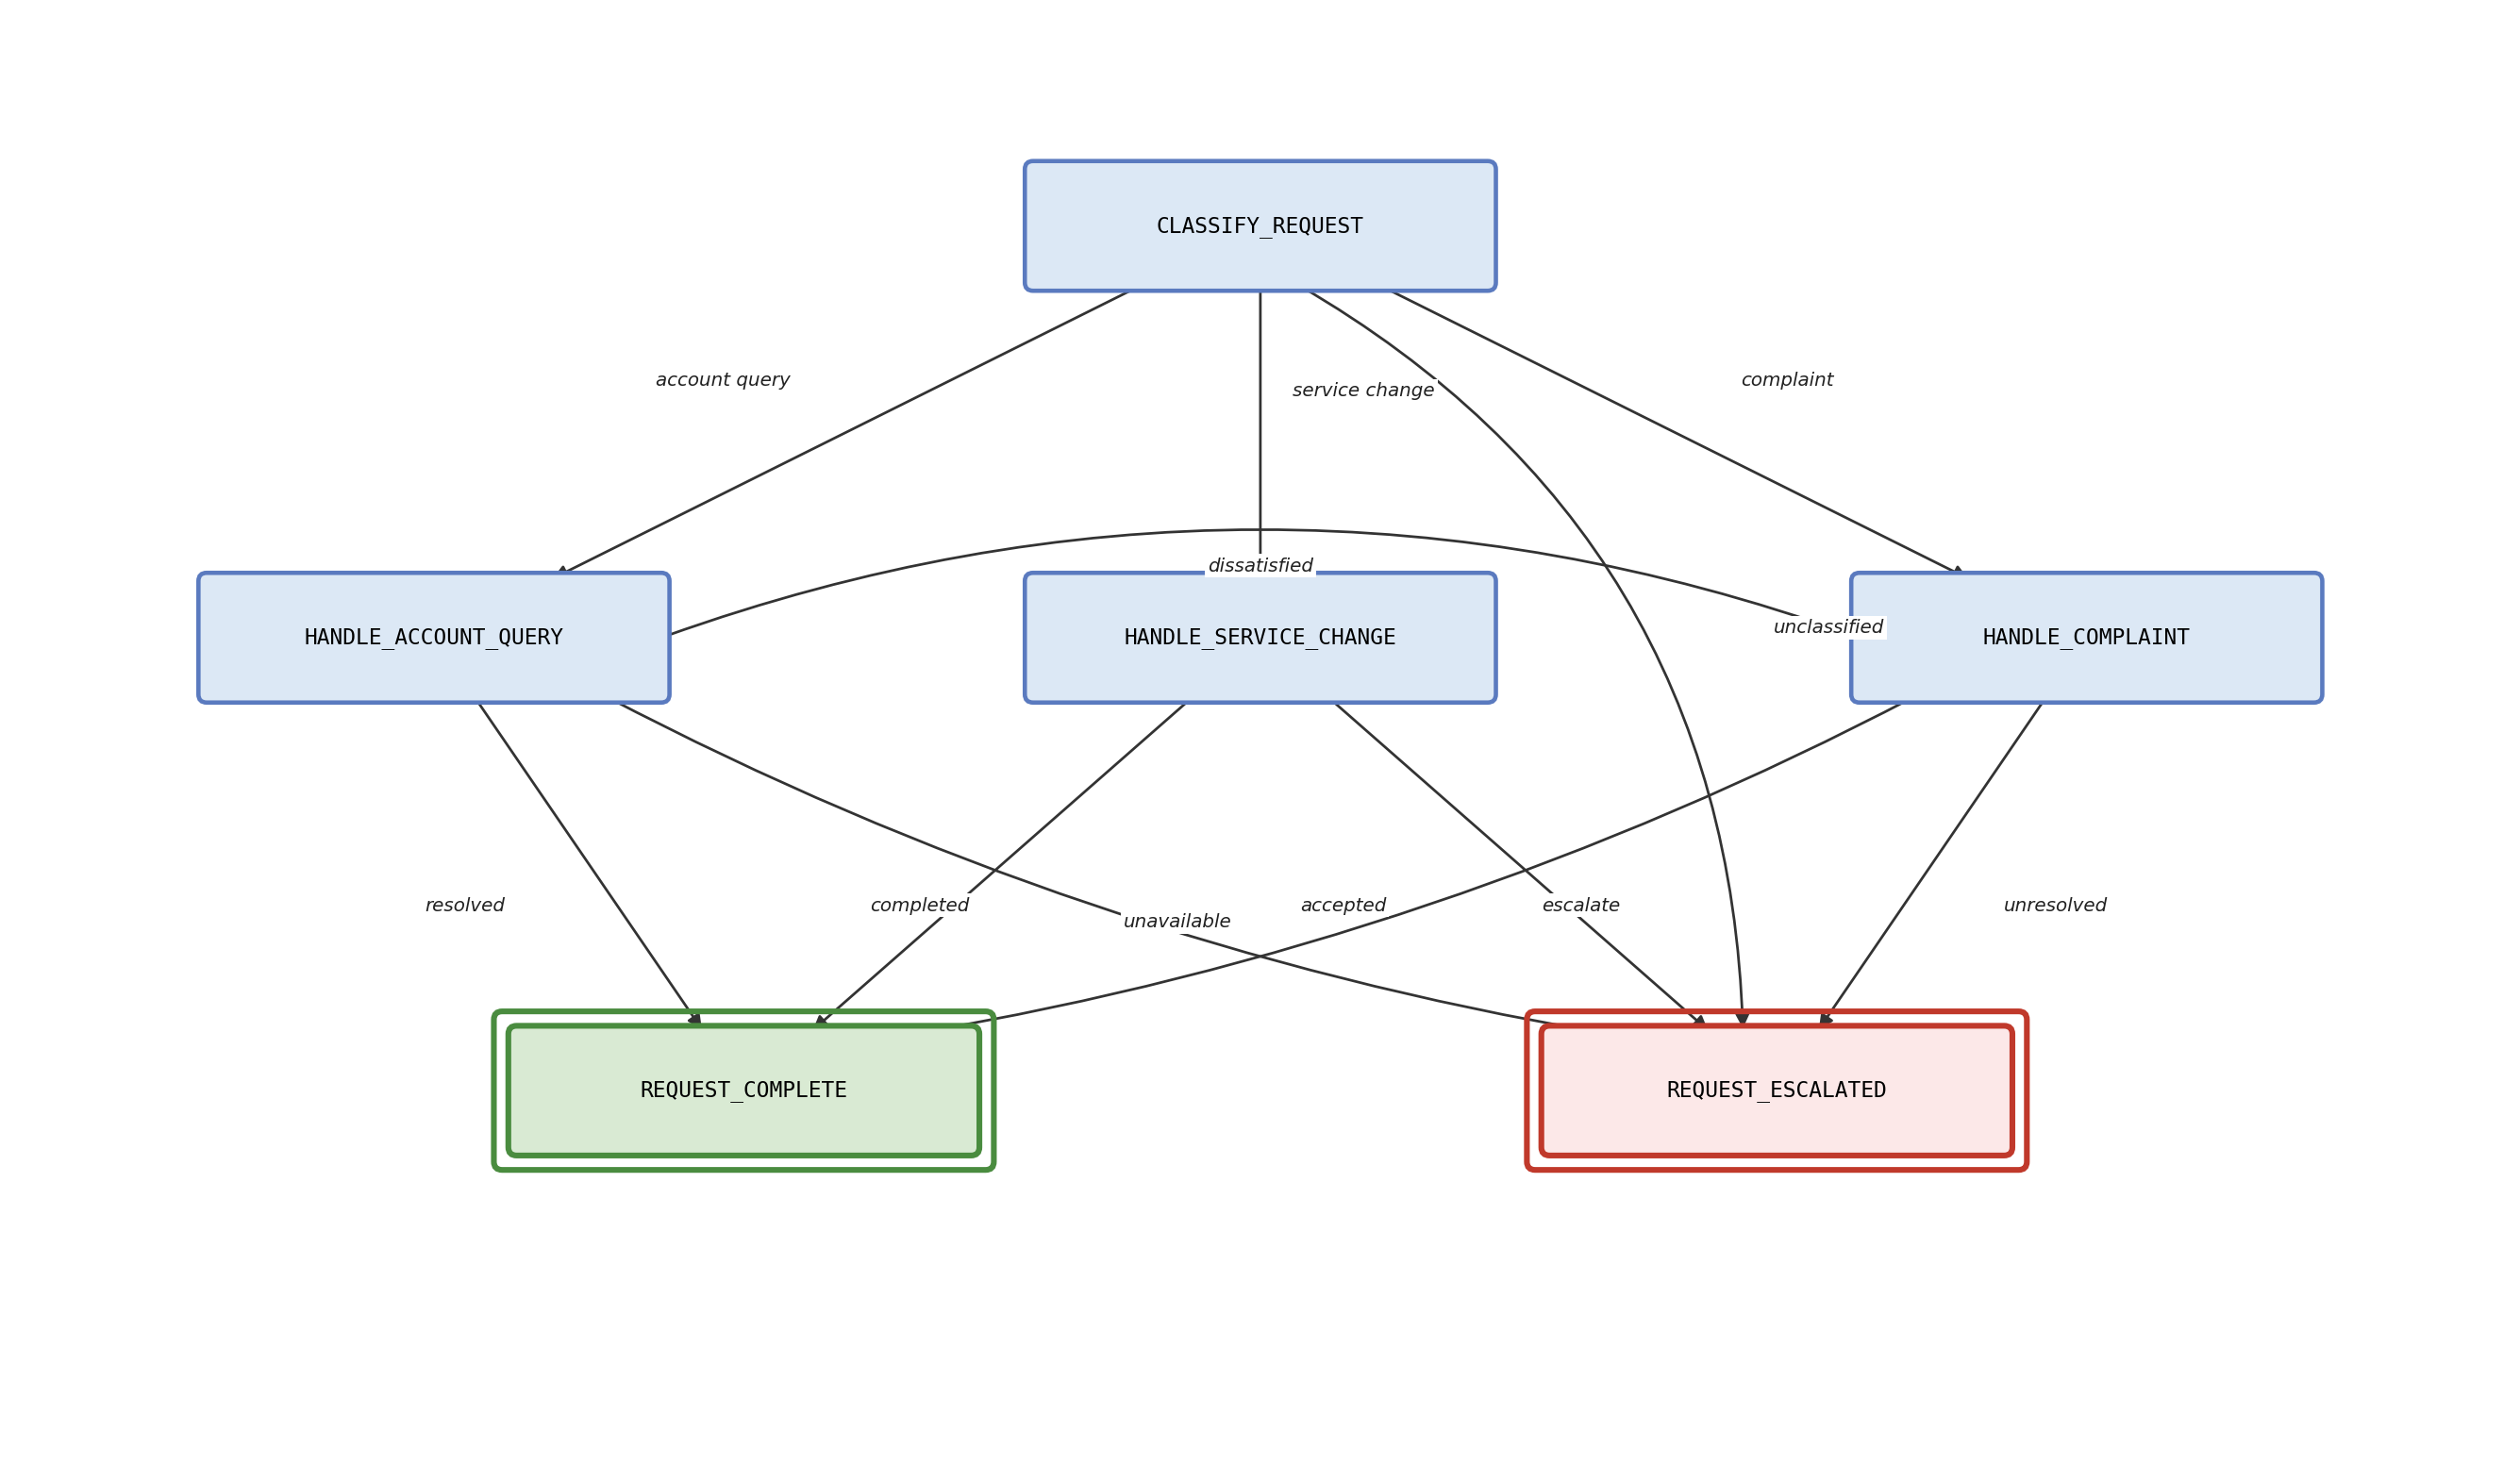
\includegraphics[width=\textwidth]{figures/workflow_diagram.png}
\caption{Directed state graph for the \texttt{SERVICE\_REQUEST} workflow
(Listing~\ref{lst:yaml}).  Blue nodes: processing states.
Green double border: success terminal (\texttt{REQUEST\_COMPLETE}).
Red double border: escalation terminal (\texttt{REQUEST\_ESCALATED}).
Every non-terminal state has at least one path to a declared terminal,
satisfying the structural reachability requirement
(Section~\ref{sec:validation}).}
\label{fig:workflow}
\end{figure*}


% ===============================================================
\bibliographystyle{IEEEtran}
\begin{thebibliography}{99}

\bibitem{dumas2018fundamentals}
M.~Dumas, M.~La~Rosa, J.~Mendling, and H.~A.~Reijers,
\textit{Fundamentals of Business Process Management}, 2nd~ed.
Springer, 2018.

\bibitem{omg2013bpmn}
Object Management Group,
``Business Process Model and Notation (BPMN) Version 2.0,''
OMG Document formal/2013-12-09, 2013. [Online]. Available:
\url{https://www.omg.org/spec/BPMN/2.0/}

\bibitem{kourani2024promoai}
H.~Kourani, A.~Berti, D.~Schuster, and W.~M.~P.~van~der~Aalst,
``Process modeling with large language models,''
in \textit{Enterprise, Business-Process and Information Systems
Modeling}, vol.~511, pp.~229--244. Springer, 2024.

\bibitem{vidgof2023bpm}
M.~Vidgof, S.~Bachhofner, and J.~Mendling,
``Large language models for business process management:
Opportunities and challenges,''
in \textit{Proc.\ BPM Forum}, LNBIP vol.~490,
pp.~107--123, Springer, 2023.

\bibitem{langgraph2024}
LangChain Inc.,
``LangGraph: Building stateful, multi-actor applications
with LLMs,'' Technical documentation, 2024. [Online]. Available:
\url{https://langchain-ai.github.io/langgraph/}

\bibitem{liu2023lost}
N.~F.~Liu, K.~Lin, J.~Hewitt, A.~Paranjape, M.~Bevilacqua,
F.~Petroni, and P.~Liang,
``Lost in the middle: How language models use long contexts,''
\textit{Trans.\ Assoc.\ Comput.\ Linguistics}, vol.~12,
pp.~157--173, 2023.

\bibitem{yao2023react}
S.~Yao, J.~Zhao, D.~Yu, N.~Du, I.~Shafran, K.~Narasimhan,
and Y.~Cao,
``ReAct: Synergizing reasoning and acting in language models,''
in \textit{Proc.\ ICLR}, 2023.

\bibitem{wang2024survey}
L.~Wang et al.,
``A survey on large language model based autonomous agents,''
\textit{Frontiers Comput.\ Sci.}, vol.~18, no.~6, 2024.

\bibitem{wu2023autogen}
Q.~Wu et al.,
``AutoGen: Enabling next-generation LLM applications via
multi-agent conversation,''
\textit{arXiv preprint arXiv:2308.08155}, 2023.

\bibitem{crewai2024}
J.~Moura,
``CrewAI: Framework for orchestrating role-playing autonomous
AI agents,'' GitHub repository, 2024. [Online]. Available:
\url{https://github.com/joaomdmoura/crewAI}

\bibitem{brady2026springdrift}
S.~Brady,
``Springdrift: An auditable persistent runtime for LLM agents,''
\textit{arXiv preprint arXiv:2604.04660}, 2026.

\bibitem{souza2025provenance}
R.~Souza et al.,
``LLM agents for interactive workflow provenance,''
in \textit{Workshops of SC'25}, ACM, 2025.
\url{https://doi.org/10.1145/3731599.3767582}

\end{thebibliography}

\end{document}
